\documentclass[conference]{IEEEtran}

\usepackage{cite}
\usepackage{amsmath,amssymb,amsfonts}
\usepackage{mathtools}
\usepackage{algorithmic}
\usepackage{graphicx}
\usepackage{textcomp}
\usepackage{xcolor}


\begin{document}


\title{Towards Exascale Computing for High Energy Physics: The ATLAS Experience at ORNL}


\author{\IEEEauthorblockN{V Ananthraj\IEEEauthorrefmark{1}, K De\IEEEauthorrefmark{2}, S Jha\IEEEauthorrefmark{3}\IEEEauthorrefmark{5},
A Klimentov\IEEEauthorrefmark{4}, D Oleynik\IEEEauthorrefmark{2}, S Oral\IEEEauthorrefmark{1}, A Merzky\IEEEauthorrefmark{3}, \\ R Mashinistov\IEEEauthorrefmark{4}, S Panitkin\IEEEauthorrefmark{4}, P Svirin\IEEEauthorrefmark{4}, M Turilli\IEEEauthorrefmark{3}, J Wells\IEEEauthorrefmark{1}, S Wilkinson\IEEEauthorrefmark{2}
}\\

\IEEEauthorblockA{\IEEEauthorrefmark{1}OLCF, Oak Ridge National Laboratory, Oak Ridge, TN, USA}
\IEEEauthorblockA{\IEEEauthorrefmark{2}Department of Physics, University of Texas, Arlington, TX, USA}
\IEEEauthorblockA{\IEEEauthorrefmark{3}Department of Electrical and Computer Engineering, Rutgers University, Piscataway, NJ, USA}
\IEEEauthorblockA{\IEEEauthorrefmark{4}Department of Physics, Brookhaven National Laboratory, Upton, NY, USA}
\IEEEauthorblockA{\IEEEauthorrefmark{5}Computational Science Initiative, Brookhaven National Laboratory, Upton, NY, USA}
}

\maketitle

\begin{abstract}


Traditionally, the ATLAS experiment at Large Hadron Collider (LHC) has utilized distributed resources as provided by the Worldwide LHC Computing Grid (WLCG) to support data distribution, data analysis and simulations.  For example, the ATLAS experiment uses a geographically distributed grid of approximately 200,000 cores continuously (250 000 cores at peak), (over 1,000 million core-hours per year) to process, simulate, and analyze its data (today’s total data volume of ATLAS is more than 300 PB). After the early success in discovering a new particle consistent with the long-awaited Higgs boson, ATLAS is continuing the precision measurements necessary for further discoveries. 
Planned high-luminosity LHC upgrade and related ATLAS detector upgrades, that are necessary for physics searches beyond Standard Model, pose serious challenge for ATLAS computing.
Data volumes are expected to increase at higher energy and luminosity, causing the storage and computing needs to grow at a much higher pace than the flat budget technology evolution (see Fig.~\ref{computing_1}).
\begin{figure}[htbp]
	\centerline{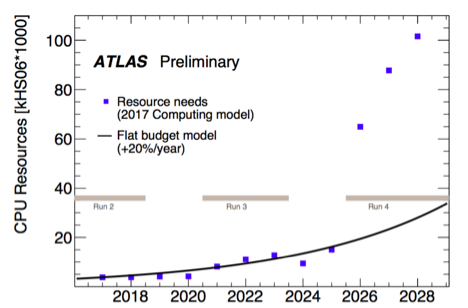
\includegraphics[width=0.5\textwidth]{hl-computing-projection.png}}
	\caption{Estimated ATLAS computing needs vs expected increase in resources on a flat budget. Gray horizontal bars depict LHC data taking periods. }
	\label{computing_1}
\end{figure}
The need for simulation and analysis will overwhelm the expected capacity of WLCG computing facilities unless the range and precision of physics studies will be curtailed.

\begin{figure}[htbp]
	\centerline{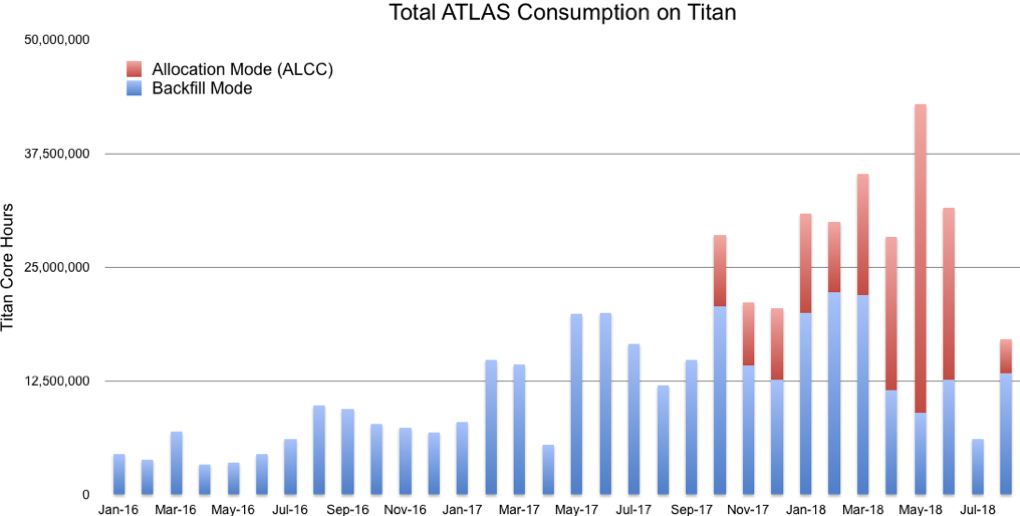
\includegraphics[width=0.5\textwidth]{total-atlas-consumption.png}}
	\caption{ATLAS  CPU consumption on Titan from January 2016 to August 2018. Blue bars correspond to resource consumption via backfill and no defined allocation, red bars - consumption using ALCC allocation. }
	\label{titan1}
\end{figure}
To alleviate these challenges, over the past few years, the ATLAS experiment has been investigating the implications of using high-performance computers -- such as those found at Oak Ridge Leadership Computing Facility (OLCF). This steady transition is a consequence of application requirements (e.g., greater than expected data production), technology trends and software complexity.  Specifically, the DOE ASCR and HEP funded the BigPanDA project provided the first important demonstration of the capabilities that a workload management system (WMS) can have on improving the uptake and utilization of supercomputers from both application and systems points of view.

We quantify the impact of this sustained and steady uptake of supercomputer resources via BigPanDA: From January 2017 to September 2018, Big Panda has enabled the utilization of ~400 Million Titan core hours primarily via Backfill mechanisms 275M, but also through regular “front end” submission as part of the ALCC project (ASCR Leadership Computing Challenge) 125M.  Fig.~\ref{titan1} shows monthly core-hour consumption on Titan by ATLAS jobs.


This non-trivial amount of 400 million Titan core hours has resulted in 920 million simulated events delivered to ATLAS physicists for analysis. ~3-5\% of all of ATLAS compute resources now provided by Titan; other DOE supercomputers also provide significant compute allocations.

In spite of these impressive numbers, there is a need to further improve the uptake and utilization of current and future supercomputing resources in order to meet ATLAS computing challenges in high luminosity regime. 

In this short paper, we will outline how we have steadily made the ATLAS project ready for the exascale era.

Our approach to the exascale involve the BigPanDA workload management system.
BigPanDA is responsible for coordination of tasks, orchestration of resources and
job submission and management. Historically, BigPanDA was used to for workload
management across multiple distributed resources on the WLCG. 
We describe the changes to the BigPanDA software system needed to enable it to utilize
Titan supercomputer. 
These enhancements include development of the new modes of resource federation (Harvester), task
execution systems (next-generation execution) as well as new applications and
communities. 

Harvester is intended to operate as a universal resource-facing service in BigPanDA,
capable of working with different types of computing resources - Grid sites, clouds and supercomputers.
Harvester provides for flexible scheduling of  job execution and asynchronous data transfer to and from the controlled resource.
Harvester has modular multi-threaded design to support heterogeneous resources and to accommodate for special workflows requirements.
\begin{figure}[htbp]
	\centerline{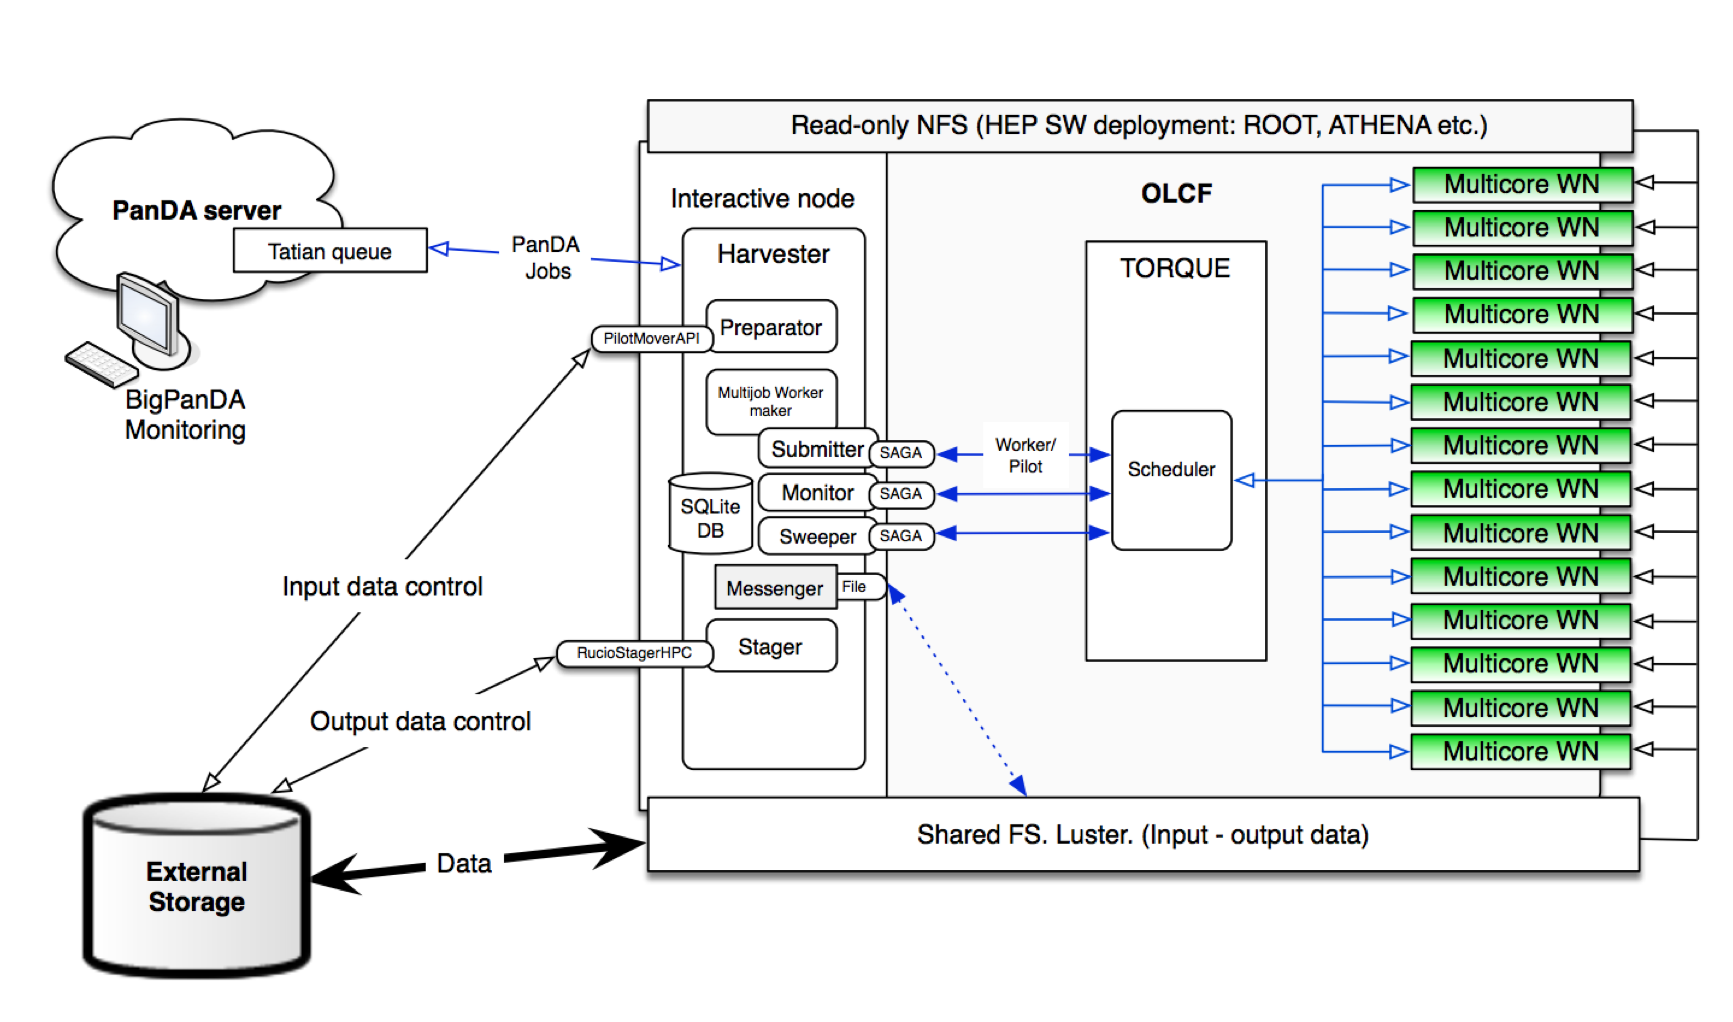
\includegraphics[width=0.5\textwidth]{harvester-on-titan.png}}
	\caption{Schematic view of Harvester deployment on Titan supercomputer at OLCF. }
	\label{harvester}
\end{figure}
We will describe our experience with Harvester installation on Titan and running of ATLAS detector simulation.

The next generation executor (NGE) is a prototype of a pilot system capable
running on Titan. By design, NGE separates workload management, resource
acquisition, and resource management capabilities, enabling multilevel
scheduling and late binding of workloads to resources. NGE submits a job on
Titan to acquire resources and, once the job is scheduled, bootstraps a pilot
agent on those resources. This agent pulls the tasks provided by Harvester
and schedules them for execution on the acquired resources. The pulling and
scheduling of these tasks are independent from Titan's batch system: tasks
run concurrently on all the available resources and, when a task completes,
another task is immediately scheduled for execution, until the resources'
walltime is exhausted. In this way, NGE enables the execution of multiple
`generations' of tasks without interfering with the machines policies for
resource allocation and utilization.

\begin{figure}[htbp]
	\centerline{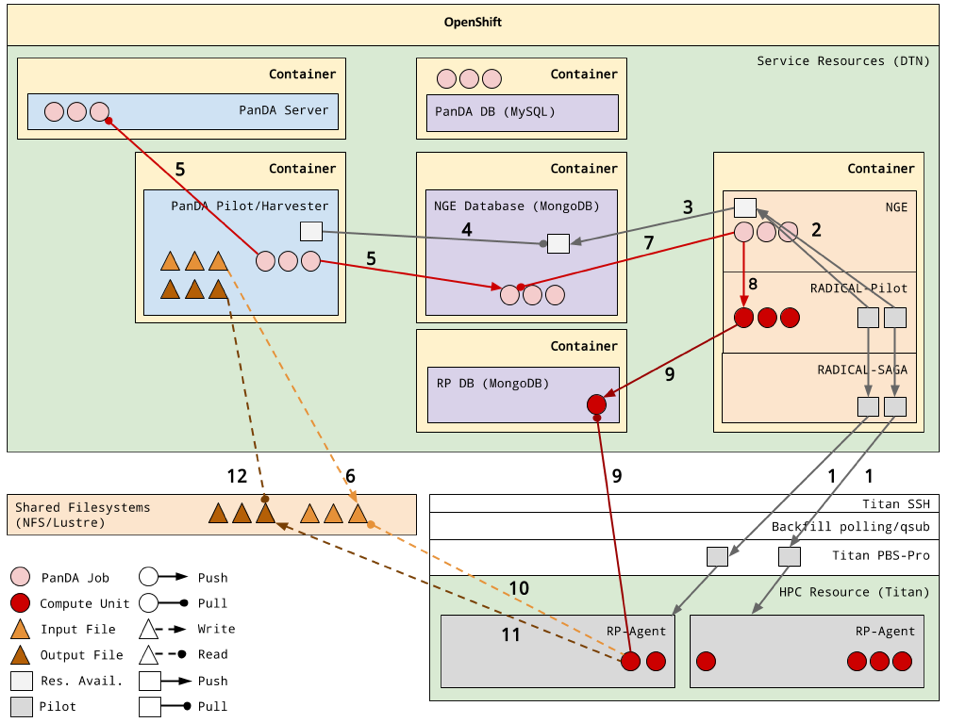
\includegraphics[width=0.5\textwidth]{nge.png}}
	\caption{NGE/PanDA Server Architecture. Communication between the two systems is mediated via a dedicated database. Communication with the database is performed via a REST interface exposed by NGE.}
	\label{nge}
\end{figure}

Currently, when a set of simulations ends, the batch job also ends,
independent of whether more walltime would still be available. With NGE,
additional payloads could be executed to utilize all the available walltime,
while avoiding further job packaging and submission overheads. Multiple
generations would also relax two assumptions of the current execution model:
knowing the number of simulations before submitting the batch job, and having
a fixed number of events per simulation. Pilots would enable the scheduling
of simulations independently from whether they were available at the moment
of submitting the pilot.

Another important capability of NGE is to separate the management of the
execution of a workflow from the code that the workflow executes on the HPC
resources. This means that NGE will be agnostic towards executing simulations
of the Geant4 based workflows and, for example, event generators. We will
describe NGE installation on Titan, performance tests as well as current
status of integration between Harvester and NGE.

We will then describe how architectural, algorithmic and software changes
have also been addressed by ATLAS computing. In particular we will describe a
project aimed at adaptation of ATLAS codes to the next generation Summit
supercomputer that is expected to be commissioned in late 2018 at ORNL. ATLAS
software framework consists of millions lines of code in hundreds of modules
and components developed by the ATLAS collaboration as well as multiple open
source packages developed outside of ATLAS. The framework is also sensitive
to the operating system libraries and hence the complete recompilation
represents a significant technical challenge. Up to now, ATLAS software
releases are built at CERN for Linux x86 architecture and after validation
the binaries are distributed to Grid computing sites. These procedures will
not work for Summit due binary incompatibility between Power9 and x86
architectures and current absence of Power9 compatible build platforms at
CERN. In order to overcome this problem we performed ATLAS software
recompilation for Power9 target using  Summitdev computer at ORNL as a build
platform.

NGE will play a key role in the adoption of Summit. Its design isolates the
capabilities required to acquire resources on Summit from those used to
submit a workload for execution. In this way, porting NGE to Summit requires
enabling job submission via Summit's IBM Spectrum Load Sharing Facility (LSF)
batch system, the tailoring of the pilot agent's scheduler to the
heterogeneous architecture of Summit work nodes, and the development of an
executor based on JSRUN, the job launcher developed by IBM for the Oak Ridge
and Livermore CORAL systems. The interface between Harvester and NGE, and the
code that enables workload management within NGE will need no changes.
Further, once Summit will be supported, NGE will enable Harvester to
concurrently submit workloads to both to Titan and Summit, without any
additional development overhead.

We will conclude with outlining plans for future improvements to BigPanDA to
make it ready for efficient use of the pre-exascale machines such as Summit.



\end{abstract}

\end{document}
